\documentclass{standalone}

\makeatletter

\usepackage{tikz}
\usetikzlibrary{decorations.markings}

\makeatother

\begin{document}
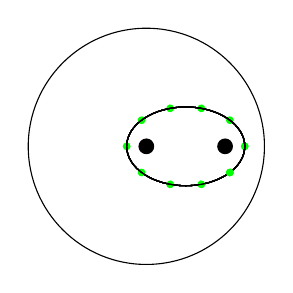
\begin{tikzpicture}[
  tangent/.style={
    decoration={ markings,% switch on markings
      mark=
          at position #1
          with {
            \coordinate (tangent point-\pgfkeysvalueof{/pgf/decoration/mark info/sequence
              number}) at (0pt,0pt);
            \coordinate (tangent unit vector-\pgfkeysvalueof{/pgf/decoration/mark info/sequence
              number}) at (1,0pt);
            \coordinate (tangent orthogonal unit
            vector-\pgfkeysvalueof{/pgf/decoration/mark info/sequence number}) at (0pt,1);
          }
        },
        postaction=decorate
      },
      use tangent/.style={
        shift=(tangent point-#1),
        x=(tangent unit vector-#1),
        y=(tangent orthogonal unit vector-#1)
      },
      use tangent/.default=1
      ]

     \begin{scope}
       %\clip (0,0) circle (1.5);
       \foreach \x in {0,0.1,0.2,0.3,...,1.1}{
         \draw [tangent=\x] (0.5,0) ellipse (0.75 and 0.5);
         % (-0.25,0) to [out=-90,in=-90] (1.25,0) to [out=90,in=90] (-0.25,0);
         \fill[use tangent,green] (0,0) circle (0.05);
       }
     \end{scope}
     \draw (0,0) circle (1.5);
     \fill (0,0) circle (0.1) (1,0) circle (0.1);
\end{tikzpicture}
\end{document}